\documentclass[a4paper, 10pt, final, garamond]{book}
\usepackage{cours-preambule}
\graphicspath{{./figures/}}

\makeatletter
\renewcommand{\@chapapp}{Contr\^ole de connaissances}
\makeatother

% \toggletrue{student}
% \HideSolutionstrue
% \toggletrue{corrige}
\renewcommand{\mycol}{black}

\begin{document}
\setcounter{chapter}{17}

\settype{enon}
\settype{solu}

\chapter{Particules chargées et structure de la matière\ifstudent{ (10')}}

\begin{enumerate}[label=\sqenumi]
	\nitem{3}%
	Donner l'expression de la force de \textsc{Lorentz}. Montrer que la force
	magnétique ne modifie pas la vitesse d'une particule chargée en calculant la
	puissance de la force de \textsc{Lorentz}.
	\smallbreak
	\vspace{-15pt}
	\psw{
		\[
			\Ff \stm{=} q \left( \Ef + \vf \wedge \Bf \right)
			\Ra
			\Pc(\Ff) = q \left( \Ef + \vf \wedge \Bf \right)\cdot \vf
			= q\Ef\cdot\vf +
			q\underbracket[1pt]{\underbracket[1pt]{\vf\wedge\Bf}_{\perp\vf}\cdot\vf}_{=0}
			\Lra
			\boxed{\Pc(\Ff) \stm[-1]{=} q\Ef\cdot\vf} \stm{=} \dv{\Ec_c}{t}
		\]
	}
	\vspace{-15pt}
	\nitem{11}%
	\noindent
	\begin{minipage}[t]{.70\linewidth}
		Soit une particule de charge $q > 0$ et de masse $m$ assimilé à un point
		matériel M, arrivant avec la vitesse $\vfo = v_0\ux$ dans un champ $\Bf =
			B\uz$. On travaille en coordonnées cartésiennes dans le référentiel du
		laboratoire supposé galiléen, avec $\OM(0) = \of$. \textbf{Faire un schéma
			puis le bilan des forces et montrer que la trajectoire est circulaire}.
		Donner les rayon et pulsation cyclotron et compléter le schéma. On ne
		cherchera pas à déterminer les équations horaires de $x(t)$ et $y(t)$.
	\end{minipage}
	\hfill
	\begin{minipage}[t]{.28\linewidth}
		\vspace{-20pt}
		\begin{center}
			\sswitch{
				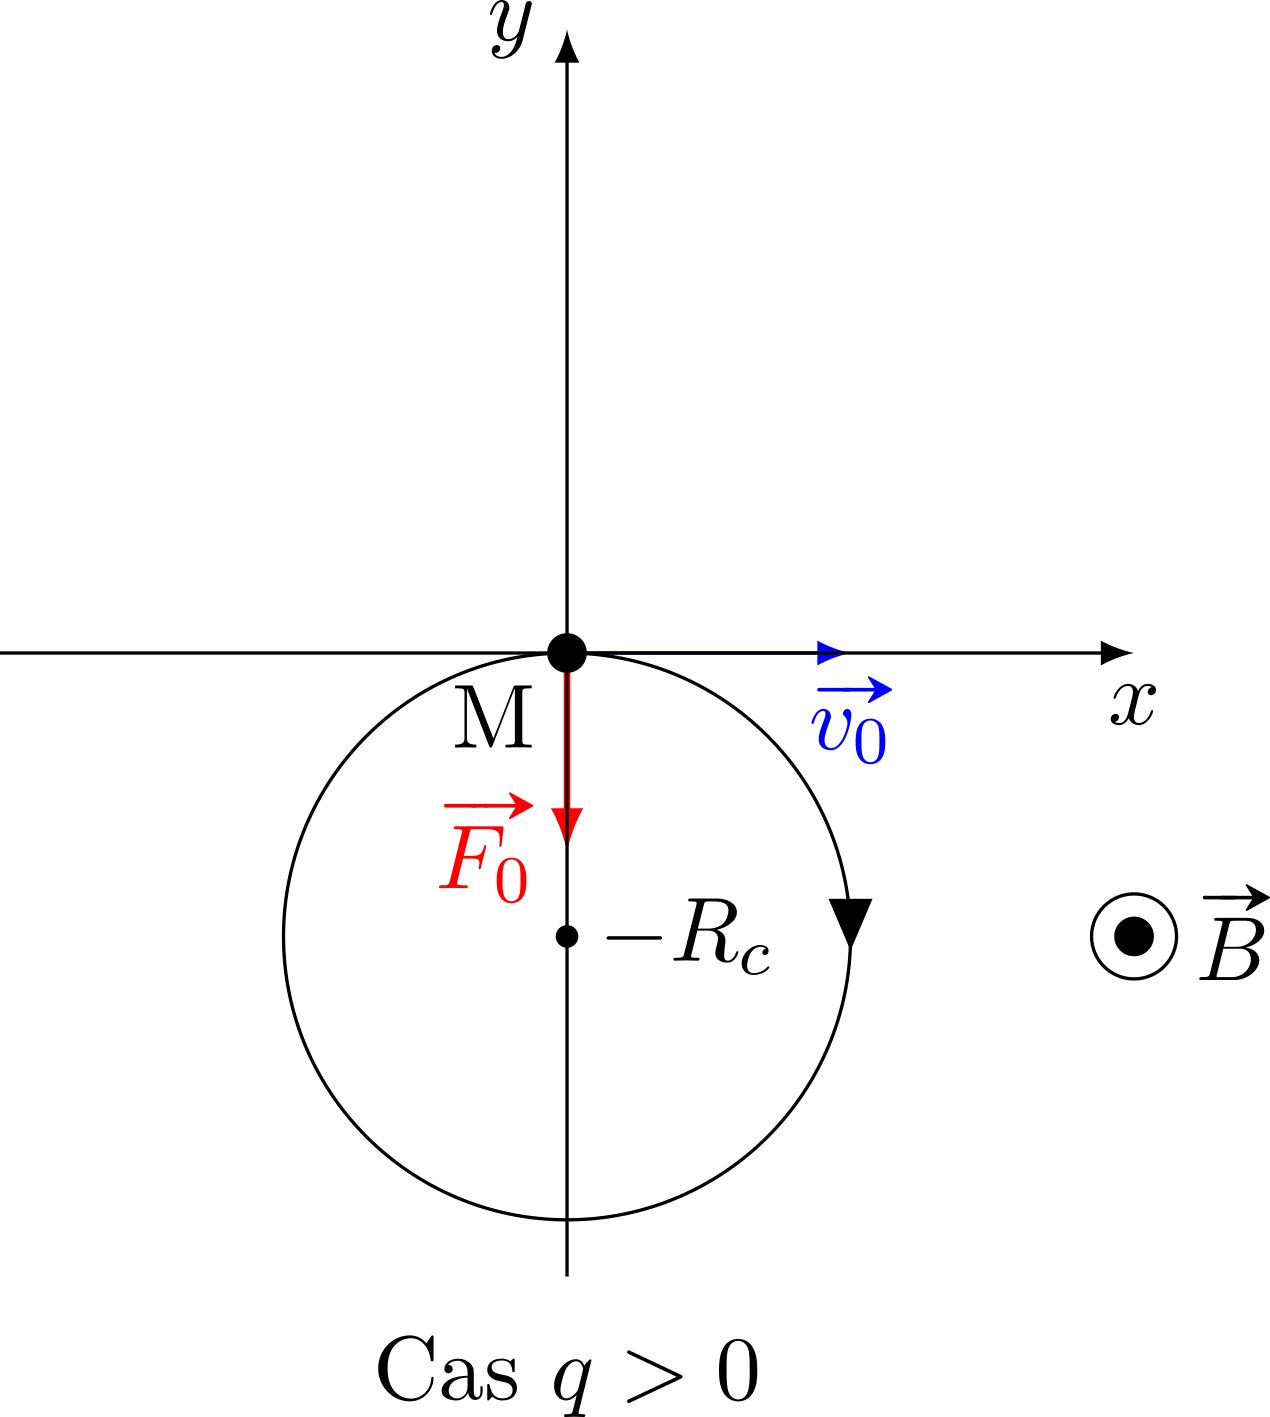
\includegraphics[width=3cm, draft=true]{chp_B-cercleqpos}
			}{
				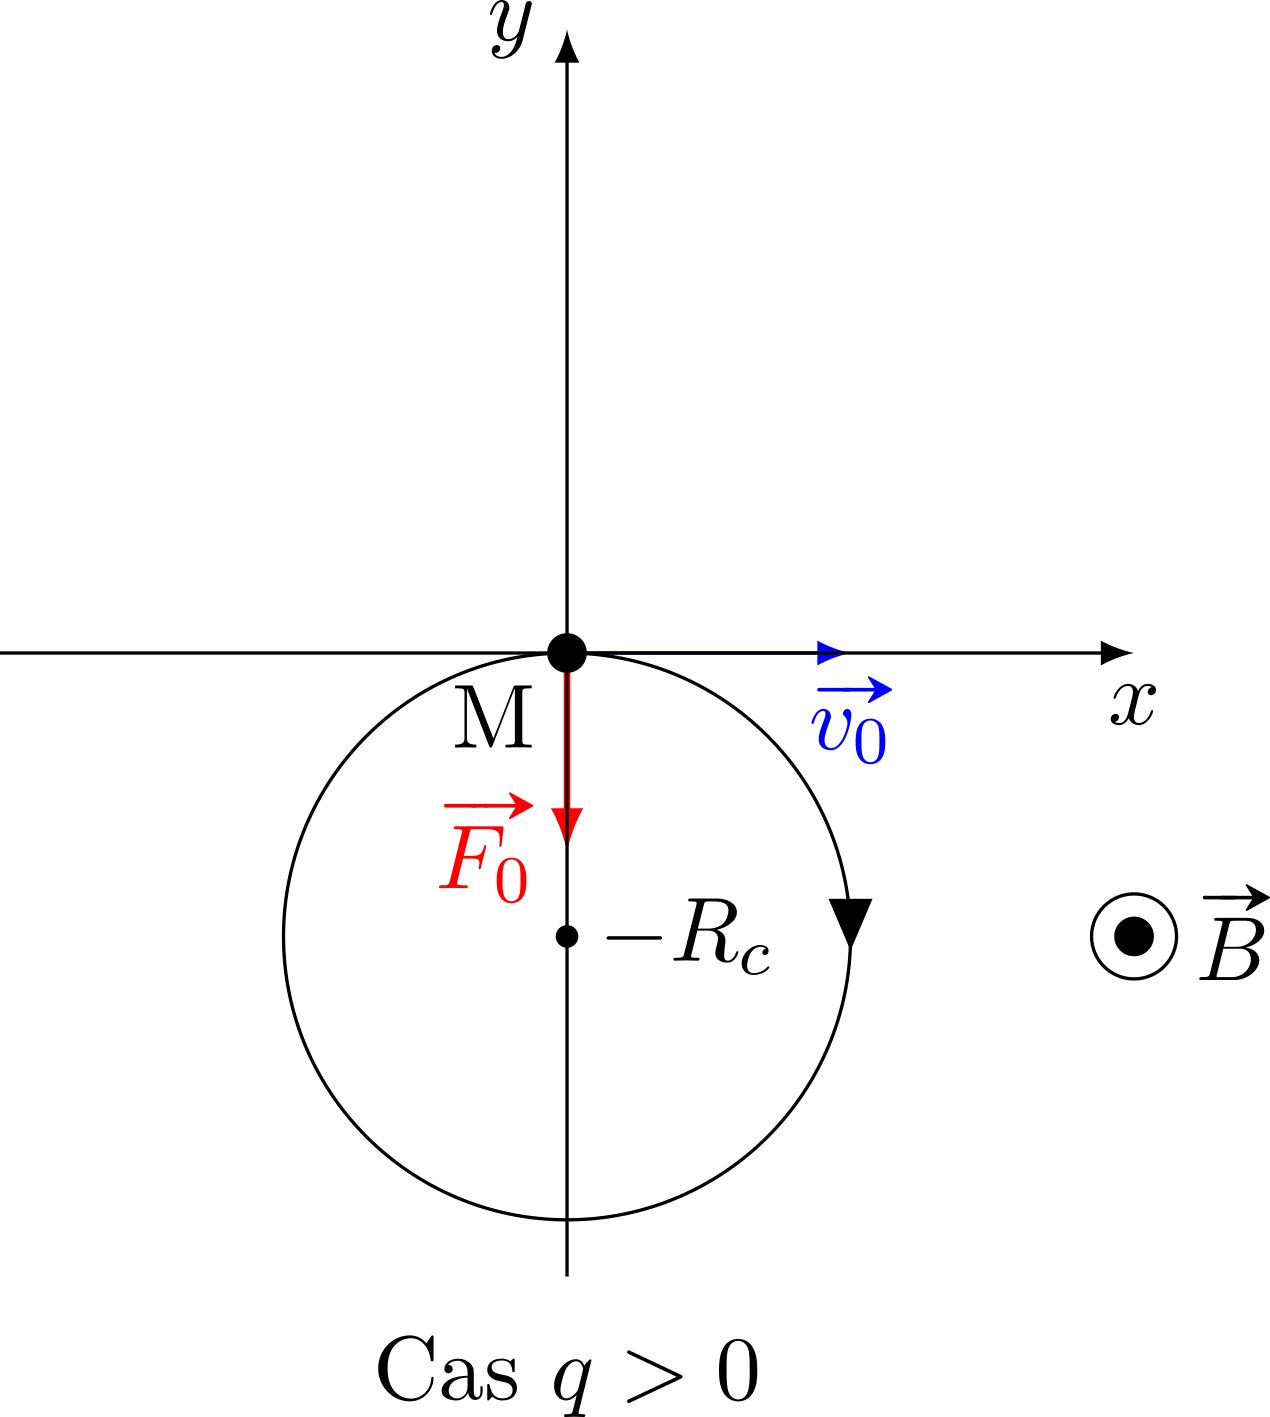
\includegraphics[width=3cm]{chp_B-cercleqpos}
			}
			\captionof{figure}{Schéma \protect\pt{2}}
		\end{center}
	\end{minipage}
	\begin{isd}
		\psw{
			\begin{gather*}
				\begin{array}{ll}
					\textbf{Poids}            & \text{négligeable \pt{1} \textbf{devant} }\Ff    \\
					\textbf{Force magnétique} & \Ff = q\vf\wedge\Bf \stm{=} q\yp B\ux -q\xp B\uy
				\end{array}\\
				m\af \stm[-1]{=} \Ff \Lra
				\left\{
				\begin{aligned}
					m\xpp & = q\yp(t)B  \\
					m\ypp & = -q\xp(t)B \\
					m\zpp & = 0
				\end{aligned}
				\right.
				\Lra
				\left\{
				\begin{aligned}
					\xpp(t) & = \frac{qB}{m}\yp(t)  \\
					\ypp(t) & = -\frac{qB}{m}\xp(t) \\
					\zpp(t) & = 0
				\end{aligned}
				\right.
				\\\Ra \pt{1}
				\left\{
				\begin{aligned}
					\xp(t) & = \frac{qB}{m}y(t) + v_0 \\
					\yp(t) & = -\frac{qB}{m}x(t) + 0  \\
					\zp(t) & = 0
				\end{aligned}
				\right.
			\end{gather*}
		}
		\tcblower
		\psw{
			\begin{gather*}
				\beforetext{TPC $\Ra$}
				\Ec_c = \cte \Lra \xp(t)^2 + \yp(t)^2 \stm{=} \cte = v_0{}^2
				\\\Lra
				\left(\frac{qB}{m}y(t) + v_0\right)^2 + \left(-\frac{qB}{m}x(t)\right)^2 =
				v_0{}^2
				\\\Lra
				\boxed{
					\left(y + \frac{v_0}{\w_c}\right)^2 + (x)^2 \stm[-1]{=}
					\left( \frac{v_0}{\w_c} \right)^2
				}
			\end{gather*}
			C'est l'équation d'un cercle \pt{1}, avec $\w_c \stm[-1]{=}
				\abs{q}B/m$ la pulsation cyclotron et de rayon cyclotron $R_c =
				\frac{v_0}{\w_c} \stm[-1]{=} \frac{v_0m}{\abs{q}B}$.
		}
	\end{isd}
	\nitem{3}%
	Remplir le tableau~:
	\vspace{-25pt}
	\begin{center}
		\captionof{table}{Schémas de \textsc{Lewis} des blocs $s$ et $p$.}
		\label{tab:lewissp}
		\begin{tabular}{lcccccccc}
			\toprule
			                                                                                                                      &
			\multicolumn{2}{c}{\textbf{Bloc s}}                                                                                   &
			\multicolumn{6}{c}{\textbf{Bloc p}}
			\\ \cmidrule(lr){2-3} \cmidrule(lr){4-9}
			Colonne \pt{1}                                                                                                        & \psw{1}
			                                                                                                                      & \psw{2} & \psw{13} & \psw{14} & \psw{15} & \psw{16} & \psw{17} & \psw{18}
			\\\midrule
			Nb. é.\ valence \pt{1}                                                                                                & \psw{1} & \psw{2}  & \psw{3}  & \psw{4}  & \psw{5}  & \psw{6}  & \psw{7}  & \psw{8}
			\\\midrule
			Schéma  \pt{1}                                                                                                        &
			\psw{\Charge{[.style={fill=\sswitch{white}{black}}]0=\.}{X}}                                                          &
			\psw{\Charge{[.style={fill=\sswitch{white}{black}}]0=\.,90=\.}{X}}                                                    &
			\psw{\Charge{[.style={fill=\sswitch{white}{black}}]0=\.,90=\.,180=\.}{X}}                                             &
			\psw{\Charge{[.style={fill=\sswitch{white}{black}}]0=\.,90=\.,180=\.,270=\.}{X}}                                      &
			\psw{\Charge{[.style={fill=\sswitch{white}{black}},|style={draw=\sswitch{white}{black}}]0=\|,90=\.,180=\.,270=\.}{X}} &
			\psw{\Charge{[.style={fill=\sswitch{white}{black}},|style={draw=\sswitch{white}{black}}]0=\|,90=\|,180=\.,270=\.}{X}} &
			\psw{\Charge{[.style={fill=\sswitch{white}{black}},|style={draw=\sswitch{white}{black}}]0=\|,90=\|,180=\|,270=\.}{X}} &
			\psw{\Charge{[.style={fill=\sswitch{white}{black}},|style={draw=\sswitch{white}{black}}]0=\|,90=\|,180=\|,270=\|}{X}}
			\\\bottomrule
		\end{tabular}
	\end{center}
	\nitem{4}%
	Qu'est-ce que l'électronégativité~? Comment augmente-t-elle dans une ligne et
	une colonne de la classification périodique~? Déterminer le moment dipolaire
	de l'eau connaissant $\mu_{\ce{O-H}} = \SI{1.51}{D}$ et $(\widehat{\ce{HOH}})
		= \ang{104.45}$.
	\smallbreak
	\begin{isd}
		\psw{
			L'électronégativité traduit la tendance d'un élément à attirer les
			électrons \pt{1} d'une liaison chimique~: plus $\chi$ est grand, plus
			un élément attire à lui les électrons.
			\smallbreak
			Elle augmente de bas en haut  dans une colonne, et de gauche à droite
			\pt{1} dans une ligne. Ainsi dans $\ce{O-H}$, comme $\chi_{\ce{O}} >
				\chi_{\ce{H}}$, on a un moment dipolaire de \ce{O} vers \ce{H}~:
		}
		\tcblower
		\begin{center}
			$\vcenter{\hbox{
						\psw{
							\cfig{
								\lewis{13,O}
								(-[@{d}:-37.775]H)
								(-[@{g}:217.775]H)
							}
							\chemmove[to-to]{
								\draw
								(g) to[bend right]
								node [midway, below] {\ang{104.45}}
								(d)
								;}
						}
					}}$
			\psw{$\stm{\Lra}$}
			$\vcenter{\hbox{
						\sswitch{
							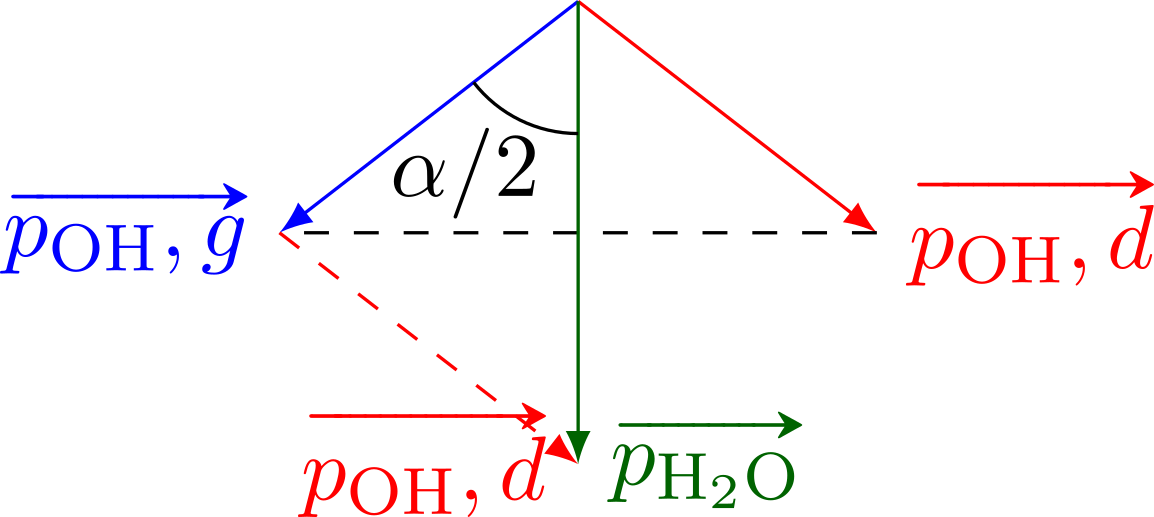
\includegraphics[scale=.8, draft=true]{pH2O}
						}{
							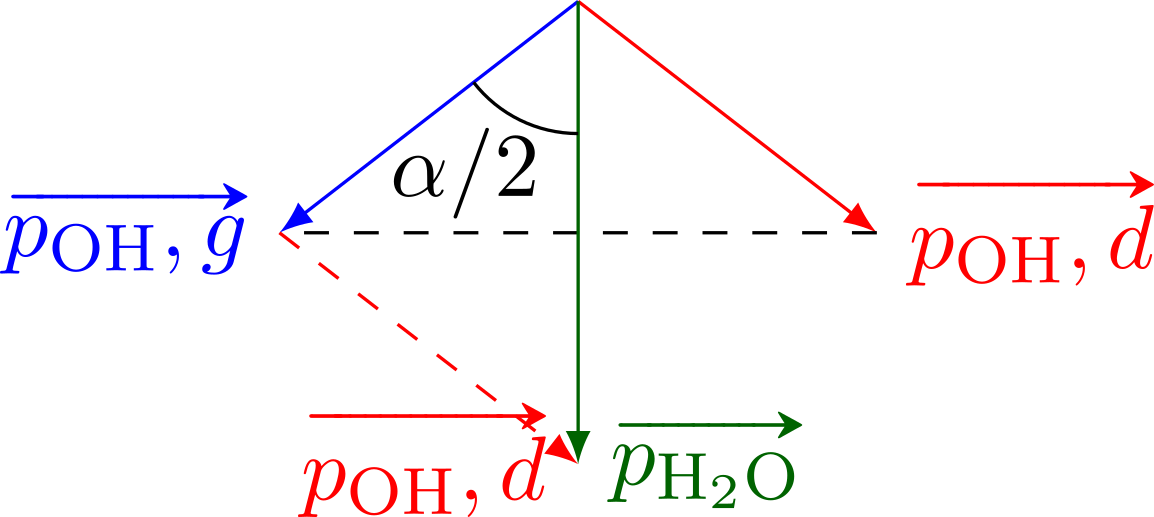
\includegraphics[scale=.8]{pH2O}
						}
					}}$
		\end{center}
		\psw{
			\begin{gather*}
				\beforetext{On trouve}
				\cos(\frac{\a}{2}) = \frac{\mu_{\ce{H2O}}/2}{\mu_{\ce{OH}}}
				\\\Lra
				\boxed{\mu_{\ce{H2O}} = 2\mu_{\ce{OH}}\cos(\a/2) \stm[-1]{=} \SI{1.85}{D}}
			\end{gather*}
		}
		\vspace{-15pt}
	\end{isd}
	\ifstudent{
		\begin{tikzpicture}[remember picture, overlay]
			\node[anchor=north west, align=left]
			at ([shift={(1.4cm,0)}]current page.north west)
			{\\[5pt]\Large\bfseries Nom~:\\[10pt]\Large\bfseries Prénom~:};
			\node[anchor=north east, align=right]
			at ([shift={(-1.5cm,-17pt)}]current page.north east)
			{\Large\bfseries Note~:\hspace{1cm}/20};
		\end{tikzpicture}
	}
\end{enumerate}
\end{document}
